\section{Escalamiento de Impedancia}

\subsection{Análisis del Circuito Prototipo}
Para iniciar el estudio, se analizó el circuito mostrado en la figura \ref{fig:circuito_orig}, el cual es alimentado por una fuente de voltaje alterno $V_1 = 120 \, V_{rms}$ a una frecuencia de $60 \, Hz$. Los valores de los componentes para este prototipo inicial son:
\begin{itemize}
	\item \textbf{Resistencias:} $R_1 = 20 \, k\Omega$, $R_2 = 300 \, \Omega$
	\item \textbf{Inductancia:} $L_1 = 1000 \, \mu H$
	\item \textbf{Capacitancia:} $C_1 = 1000 \, pF$
\end{itemize}

\begin{figure}[H]
	\centering
	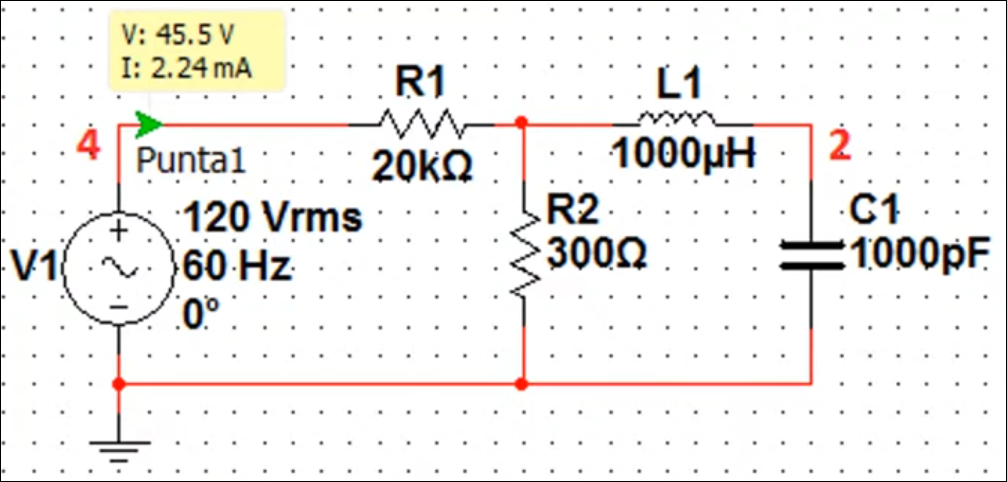
\includegraphics[width=0.7\linewidth]{assets/img/circuito_v1_1.png}
	\caption{Configuración del circuito prototipo.}
	\label{fig:circuito_orig}
\end{figure}

\subsubsection{Obtención de la Función de Transferencia}
Se definió la función de transferencia como la relación entre el voltaje en el capacitor ($V_{out}$) y el voltaje de la fuente ($V_{in}$), expresada como $H(s) = \frac{V_2}{V_4}$. Utilizando el método de mallas en el dominio de la frecuencia ($s$):

Definiendo las impedancias: $Z_{R1} = R_1$, $Z_{R2} = R_2$, $Z_L = sL_1$, $Z_C = \frac{1}{sC_1}$.
Las ecuaciones de malla resultantes son:
\begin{enumerate}
	\item $(R_1 + R_2)I_1 - R_2 I_2 = V_{in}$
	\item $-R_2 I_1 + (R_2 + sL_1 + \frac{1}{sC_1})I_2 = 0$
\end{enumerate}

Al resolver para la corriente de la segunda malla ($I_2$) y multiplicar por la impedancia del capacitor ($Z_C$), la función de transferencia queda definida por la estructura:
\begin{equation}
	H(s) = \frac{R_2}{s^2 C_1 L_1 (R_1 + R_2) + s (C_1 R_1 R_2 + L_1) + (R_1 + R_2)}
\end{equation}

\subsubsection{Resultados de la Simulación Inicial}
En la simulación a frecuencia única ($60 \, Hz$), se registraron los siguientes valores de operación:
\begin{itemize}
	\item \textbf{Voltaje de entrada ($V_4$):} $45.5 \, V$
	\item \textbf{Corriente de entrada ($I_{punta1}$):} $2.24 \, mA$
	\item \textbf{Impedancia de entrada ($|Z_1|$):} $20.3 \, k\Omega$ con una fase de $-95.76^\circ$.
\end{itemize}

\begin{figure}[H]
	\centering
	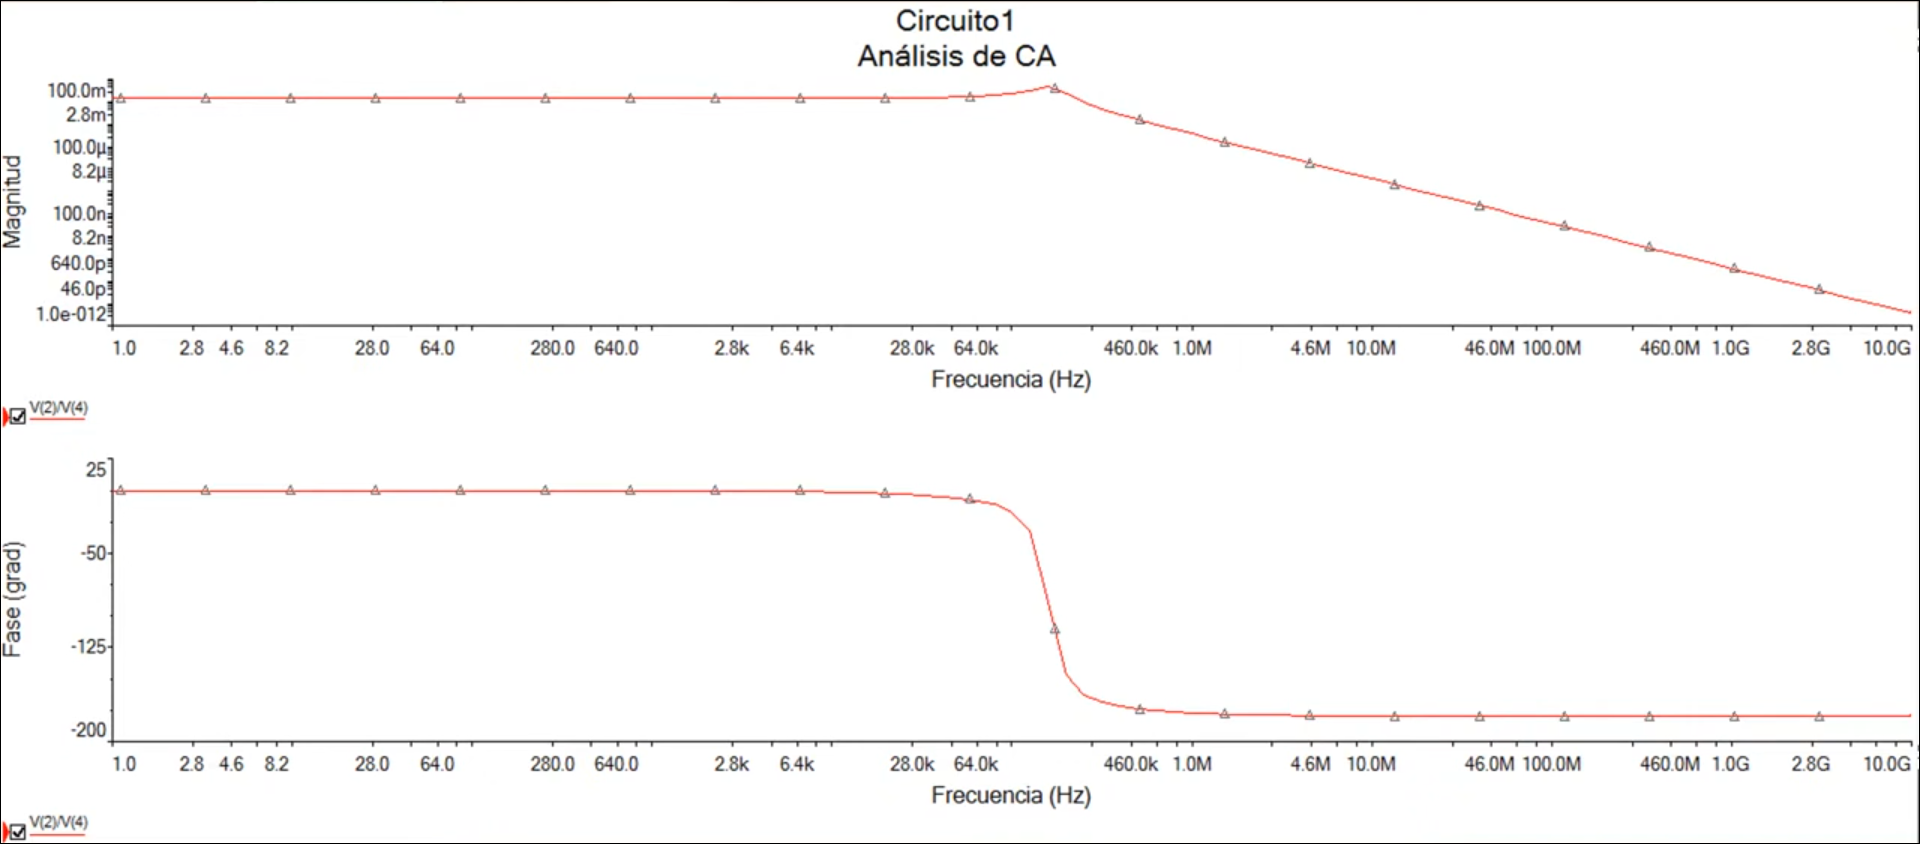
\includegraphics[width=0.8\linewidth]{assets/img/diagrama_bodeog.png}
	\caption{Diagrama de Bode.}
	\label{fig:diagrama_bodeog}
\end{figure}

\subsection{Aplicación del Escalamiento de Magnitud ($k_m = 5$)}
Se aplicó un factor de escalamiento de magnitud $k_m = 5$. El objetivo es incrementar la impedancia total de la red manteniendo la respuesta en frecuencia idéntica. Los nuevos valores se calcularon mediante las siguientes relaciones:
\begin{equation}
	R' = R \cdot k_m, \quad L' = L \cdot k_m, \quad C' = \frac{C}{k_m}
\end{equation}

Resultando en los componentes del nuevo circuito:
\begin{itemize}
	\item $R_1' = 20 \, k\Omega \times 5 = 100 \, k\Omega$
	\item $R_2' = 300 \, \Omega \times 5 = 1500 \, \Omega$
	\item $L_1' = 1000 \, \mu H \times 5 = 5000 \, \mu H$
	\item $C_1' = 1000 \, pF / 5 = 200 \, pF$
\end{itemize}

\subsubsection{Obtención de la Función de Transferencia del Circuito Escalado}
Para el circuito escalado por el factor $k_m = 5$, los componentes se transforman de acuerdo con las leyes de escalamiento de magnitud:
\begin{equation}
	R_1' = k_m R_1, \quad R_2' = k_m R_2, \quad L_1' = k_m L_1, \quad C_1' = \frac{C_1}{k_m}
\end{equation}

Sustituyendo estos nuevos valores en la estructura de la función de transferencia original:
\begin{equation}
	H'(s) = \frac{R_2'}{s^2 L_1' C_1' (R_1' + R_2') + s C_1' R_1' R_2' + (R_1' + R_2')}
\end{equation}

Al expresar cada término en función de los valores originales y el factor $k_m$:
\begin{equation}
	H'(s) = \frac{k_m R_2}{s^2 (k_m L_1) \left(\frac{C_1}{k_m}\right) (k_m R_1 + k_m R_2) + s \left(\frac{C_1}{k_m}\right) (k_m R_1) (k_m R_2) + (k_m R_1 + k_m R_2)}
\end{equation}

Simplificando los términos algebraicamente:
\begin{itemize}
	\item Término $s^2$: $(k_m L_1) \cdot \frac{C_1}{k_m} \cdot k_m(R_1 + R_2) = s^2 L_1 C_1 k_m (R_1 + R_2)$
	\item Término $s$: $\frac{C_1}{k_m} \cdot k_m R_1 \cdot k_m R_2 = s C_1 R_1 R_2 k_m$
	\item Término constante: $k_m R_1 + k_m R_2 = k_m (R_1 + R_2)$
\end{itemize}

Sustituyendo las simplificaciones y factorizando $k_m$ en el denominador:
\begin{equation}
	H'(s) = \frac{k_m R_2}{k_m [s^2 L_1 C_1 (R_1 + R_2) + s C_1 R_1 R_2 + (R_1 + R_2)]}
\end{equation}

Finalmente, al cancelar el factor $k_m$ del numerador y denominador, obtenemos:
\begin{equation}
	H'(s) = \frac{R_2}{s^2 L_1 C_1 (R_1 + R_2) + s C_1 R_1 R_2 + (R_1 + R_2)} = H(s)
\end{equation}

Este desarrollo demuestra que, aunque los valores de los componentes han cambiado para manejar menores corrientes, la relación entre el voltaje de salida y el de entrada es idéntica en el dominio de la frecuencia. Esto valida por qué los diagramas de Bode obtenidos en la simulación son superponibles.

\subsection{Verificación y Comparación de Resultados}
Tras implementar los cambios en el simulador, se realizaron nuevas mediciones para validar la teoría del escalamiento.

\begin{figure}[H]
	\centering
	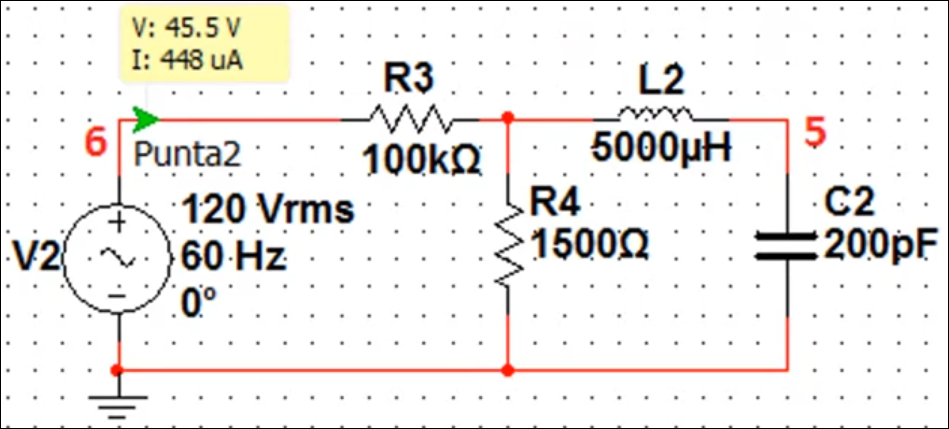
\includegraphics[width=0.8\linewidth]{assets/img/circuito_v1_2.png}
	\label{fig:circuito_escalado}
	\caption{Circuito escalado con factor $k_m = 5$.}
\end{figure}

\subsubsection{Análisis de Impedancia y Corriente}
La nueva corriente de entrada se redujo a $448 \, \mu A$ (exactamente $2.24 \, mA / 5$), mientras que el voltaje en la punta se mantuvo en $45.5 \, V$. La nueva impedancia de entrada obtenida fue:
\begin{equation}
	|Z_2| = \frac{|V_6|}{|I_{punta2}|} = 101.5 \, k\Omega
\end{equation}
Esto confirma la relación $|Z_2| = k_m \cdot |Z_1|$, ya que $101.5 \, k\Omega = 5 \cdot 20.3 \, k\Omega$. Es notable destacar que la fase de la impedancia se mantuvo invariable en $-95.76^\circ$.

\subsubsection{Validación de la Respuesta en Frecuencia}
Se compararon los diagramas de Bode de la función de transferencia original $H(s)$ frente a la escalada $H'(s)$. Como se observa en la Figura \ref{fig:bode_final}, ambos diagramas son idénticos tanto en magnitud como en fase.

\begin{itemize}
	\item \textbf{Magnitud:} Ambas curvas presentan el mismo comportamiento de filtro pasabajas con un pico de resonancia cercano a los $100 \, kHz$.
	\item \textbf{Fase:} El desplazamiento de fase inicia en $0^\circ$ y termina en $-180^\circ$ de manera idéntica en ambos circuitos.
\end{itemize}

\begin{figure}[H]
	\centering
	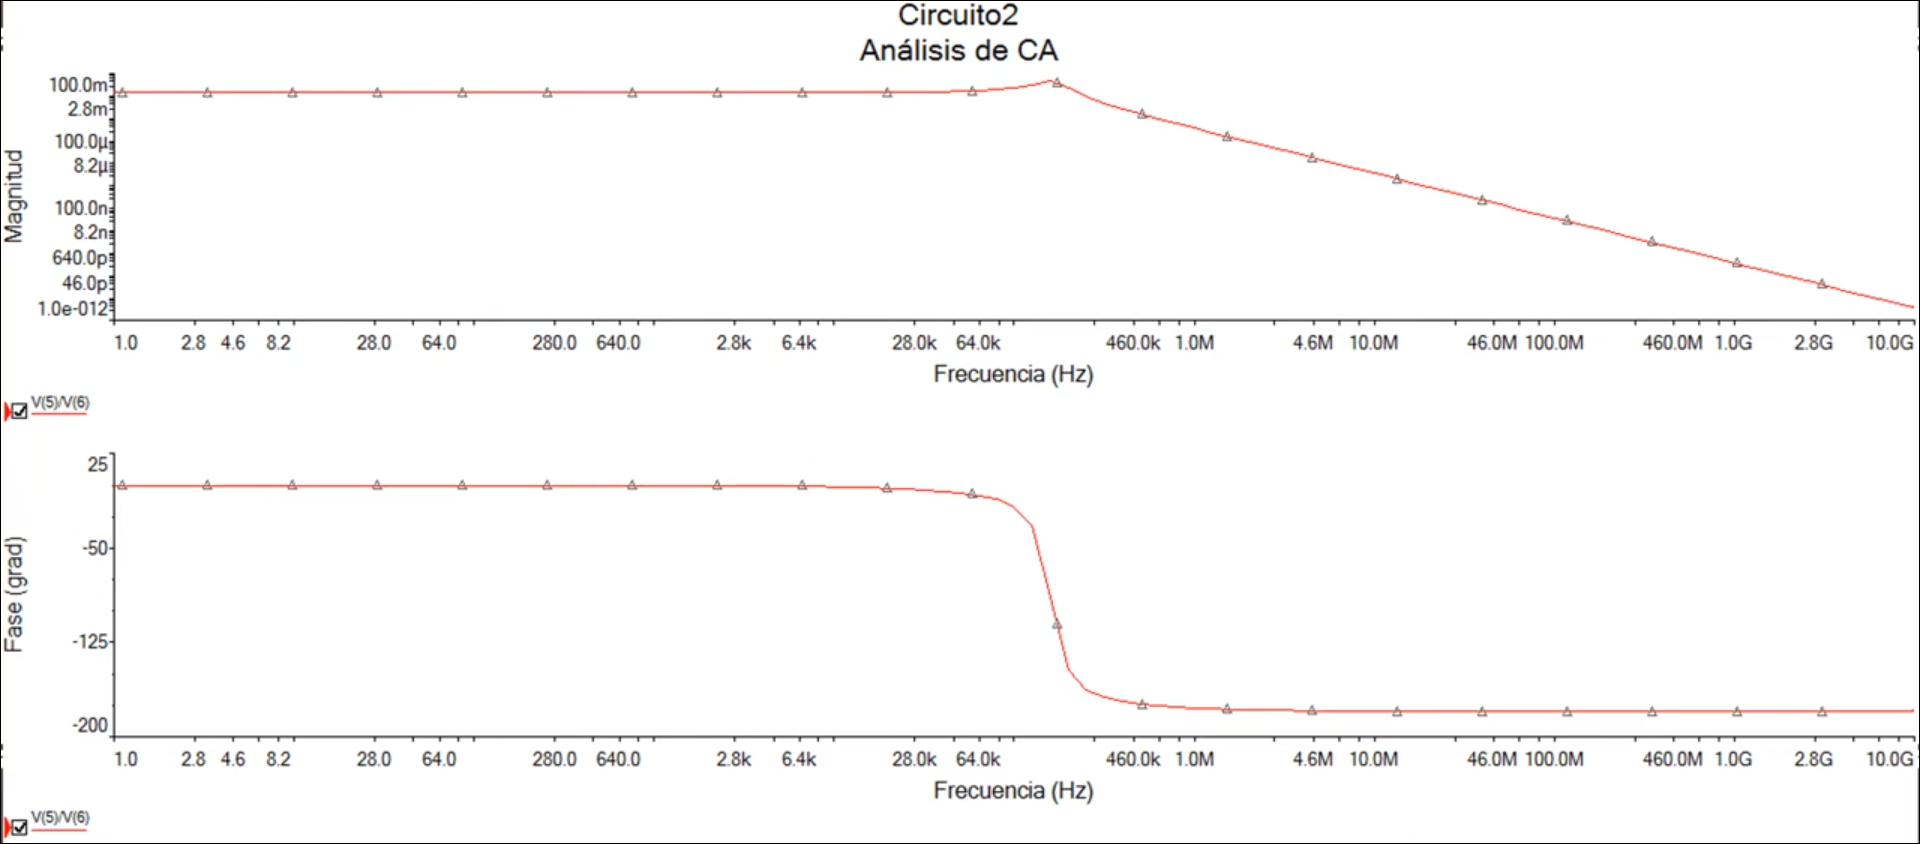
\includegraphics[width=0.8\linewidth]{assets/img/diagrama_bodeesc.png}
	\caption{Diagrama de Bode del circuito escalado. La respuesta es invariante ante el escalamiento de magnitud.}
	\label{fig:bode_final}
\end{figure}

\subsection{Conclusiones}
Los datos obtenidos se resumen en la siguiente tabla comparativa:

\begin{table}[H]
	\centering
	\begin{tabular}{|l|c|c|c|}
		\hline
		\textbf{Parámetro} & \textbf{Valor Original} & \textbf{Valor Escalado} & \textbf{Relación ($k_m$)} \\ \hline
		Resistencia ($R_1$) & $20 \, k\Omega$ & $100 \, k\Omega$ & $5$ \\ \hline
		Resistencia ($R_2$) & $300 \, \Omega$ & $1500 \, \Omega$ & $5$ \\ \hline
		Inductancia ($L_1$) & $1000 \, \mu H$ & $5000 \, \mu H$ & $5$ \\ \hline
		Capacitancia ($C_1$) & $1000 \, pF$ & $200 \, pF$ & $1/5$ \\ \hline
		Impedancia ($|Z_{in}|$) & $20.3 \, k\Omega$ & $101.5 \, k\Omega$ & $5$ \\ \hline
		Corriente ($I_{in}$) & $2.24 \, mA$ & $448 \, \mu A$ & $1/5$ \\ \hline
	\end{tabular}
	\caption{Resumen de la validación del escalamiento de impedancia.}
\end{table}

Como conclusión del escalamiento de impedancia, se demostró que permite desplazar los niveles de impedancia de una red para optimizar el consumo de corriente o adaptar componentes a valores comerciales, sin alterar en absoluto la respuesta en frecuencia ni la función de transferencia del sistema original.